% !TEX root=/home/tavant/these/manuscript/src/manuscript.tex

% \FloatBarrier

\section{Conclusion} \label{subsec-concuslion_ch4}

We observed in the \ac{2D} radial-azimuthal \ac{PIC} simulations of the exist plane of the \ac{HET} with secondary electron emission that the plasma-wall interaction was not well model.
This is certainly due to the decrease of the averaged electron temperature from the center to the wall.
We saw that the polytropic law could be used to describe this radial evolution of the electrons.
The polytropic index is observe to be close to $\gamma=1.36$ and depends weakly on the \ac{SEE} rate $\rate$.
We have noted that the primary electrons, going from the plasma center toward the wall, presented a lower polytropic index, of the order of $\gamma=1.28$.
This is consistent with the fact that the secondary electron are emitted with a Maxwellian flux distribution of temperature $\Te=2\,\volt$.

We have derived a sheath model that uses the polytropic state law to close the electron equations, and the \ac{SEE} rate is computed with the electron temperature at the wall, with a local Maxwellian hypothesis.
This model gives an equation of the potential sheath drop $\dphi$ between the sheath edge and the wall.
Depending of the electron temperature $\Teb$ and the crossover energy $\crover$, the equation can have one or three solutions.

Confronted to the \ac{PIC} simulation, the polytropic model was able to predict accurately the characteristics of the plasma-wall interaction observed in the \ac{PIC} simulation.
Using only the electron temperature and the polytropic index of the \ac{PIC} simulations, we obtain a good correspondence for both the plasma potential drop to the wall $\dphi$ and the secondary electron emission rate $\rate$ between the sheath model and the \ac{PIC} simulations.

We also observed a good correspondence between the multiple solutions of the sheath model and the sheath oscillations observed in regime {\bf II}.
Indeed, we observe that the electron temperature rises following the first branch of the solution, corresponding to regime {\bf III}.
When the electron temperature crosses the maximal temperature $\Te^1$, the sheath jumps to the third branch, which corresponds to regime {\bf I}.
In regime {\bf I}, the electron power losses increase drastically, which reduces the electron temperature until the minimum electron temperature $\Te^2$.
There, the sheath jumps back to the first branch of the solutions.

\vspace{1ex}
In the model developed here, the anisotropy between the temperature parallel and perpendicular to the magnetic field line has not been taken into account.
However, the electron flux to the wall is governed by the parallel electron temperature, while the \ac{SEE} rate depends on the two temperatures.
Hence, the electron anisotropy could modify the results of the current sheath model.
However, the radial evolution of the perpendicular electron temperature is not clearly understood.
\Cref{fig-anisotropy} shows the radial evolution of the electron temperature anisotropy  $\frac{\Te{}_{, R}}{\Te{}_{, \perp}}$ for three values of the crossover energy $\crover$

\begin{figure}[!ht]
  \centering
  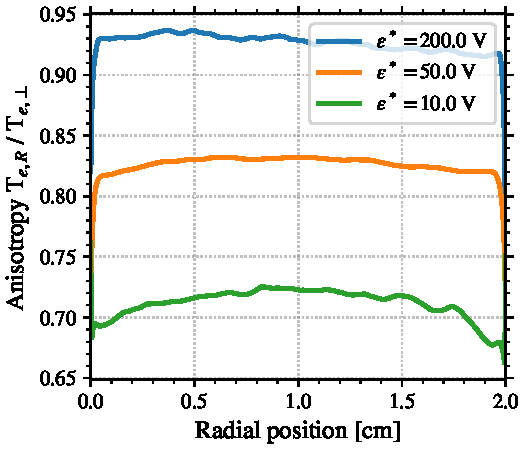
\includegraphics[width=\defaultwidth]{electron_anisotropy}
  \caption{Radial evolution of the electron anisotropy $\frac{\Te{}_{, R}}{\Te{}_{, \perp}}$ for the three values of the crossover energy $\crover=200, 50$, and $10\,\volt$.}
  \label{fig-anisotropy}
\end{figure}

We see that the electron anisotropy increases with the increases of the \ac{SEE} rate.
This is expected, as the radial losses, which increases with increasing \ac{SEE} rate, reduces the electrons with a high radial energy, without effects on the perpendicular energy.
Another observation in \cref{fig-anisotropy} is the anisotropy radial profile, which is almost uniform.
This is not consistent with the current understanding of the collisionless evolution of the electron described with the Vlasov equation developed in \cref{sec-kinetic}.
The reason of this constant anisotropy could be the azimuthal instability, which present radial structures during the saturated state.
The importance of the instability on the radial electron energy is further discussed in the next chapter, especially in \cref{sec-rheating}.





